% !TEX program = xelatex
\documentclass[a4paper,14pt,oneside,openany]{memoir}

%%% Задаем поля, отступы и межстрочный интервал %%%
\usepackage{amsmath}
\usepackage[left=30mm, right=15mm, top=20mm, bottom=20mm]{geometry} % Пакет geometry с аргументами для определения полей
\pagestyle{plain} % Убираем стандарные для данного класса верхние колонтитулы с заголовком текущей главы, оставляем только номер страницы снизу по центру
\parindent=1.25cm % Абзацный отступ 1.25 см, приблизительно равно пяти знакам, как по ГОСТ
\usepackage{indentfirst} % Добавляем отступ к первому абзацу
%\linespread{1.3} % Межстрочный интервал (наиболее близко к вордовскому полуторному) - тут вместо этого используется команда OnehalfSpacing*

%%% Задаем языковые параметры и шрифт %%%

\usepackage[english, russian]{babel}                % Настройки для русского языка как основного в тексте
\babelfont{rm}{Times New Roman}                     % TMR в качестве базового roman-щрифта

%%% Задаем стиль заголовков и подзаголовков в тексте %%%

\setsecnumdepth{subsection} % Номера разделов считать до третьего уровня включительно, т.е. нумеруются только главы, секции, подсекции
\renewcommand*{\chapterheadstart}{} % Переопределяем команду, задающую отступ над заголовком, чтобы отступа не было
\renewcommand*{\printchaptername}{} % Переопределяем команду, печатающую слово "Глава", чтобы оно не печалось
%\renewcommand*{\printchapternum}{} % То же самое для номера главы - тут не надо, номер главы оставляем
\renewcommand*{\chapnumfont}{\normalfont\bfseries} % Меняем стиль шрифта для номера главы: нормальный размер, полужирный
\renewcommand*{\afterchapternum}{\hspace{1em}} % Меняем разделитель между номером главы и названием
\renewcommand*{\printchaptertitle}{\normalfont\bfseries\centering\MakeUppercase} % Меняем стиль написания для заголовка главы: нормальный размер, полужирный, центрированный, заглавными буквами
\setbeforesecskip{20pt} % Задаем отступ перед заголовком секции
\setaftersecskip{20pt} % Ставим такой же отступ после заголовка секции
\setsecheadstyle{\raggedright\normalfont\bfseries} % Меняем стиль написания для заголовка секции: выравнивание по правому краю без переносов, нормальный размер, полужирный
\setbeforesubsecskip{20pt} % Задаем отступ перед заголовком подсекции
\setaftersubsecskip{20pt} % Ставим такой же отступ после заголовка подсекции
\setsubsecheadstyle{\raggedright\normalfont\bfseries}  % Меняем стиль написания для заголовка подсекции: выравнивание по правому краю без переносов, нормальный размер, полужирный

%%% Задаем параметры оглавления %%%

\addto\captionsrussian{\renewcommand\contentsname{Содержание}} % Меняем слово "Оглавление" на "Содержание"
\setrmarg{2.55em plus1fil} % Запрещаем переносы слов в оглавлении
%\setlength{\cftbeforechapterskip}{0pt} % Эта команда убирает интервал между заголовками глав - тут не надо, так красивее смотрится
\renewcommand{\aftertoctitle}{\afterchaptertitle \vspace{-\cftbeforechapterskip}} % Делаем отступ между словом "Содержание" и первой строкой таким же, как у заголовков глав
%\renewcommand*{\chapternumberline}[1]{} % Делаем так, чтобы номер главы не печатался - тут не надо
\renewcommand*{\cftchapternumwidth}{1.5em} % Ставим подходящий по размеру разделитель между номером главы и самим заголовком
\renewcommand*{\cftchapterfont}{\normalfont\MakeUppercase} % Названия глав обычным шрифтом заглавными буквами
\renewcommand*{\cftchapterpagefont}{\normalfont} % Номера страниц обычным шрифтом
\renewcommand*{\cftchapterdotsep}{\cftdotsep} % Делаем точки до номера страницы после названий глав
\renewcommand*{\cftdotsep}{1} % Задаем расстояние между точками
\renewcommand*{\cftchapterleader}{\cftdotfill{\cftchapterdotsep}} % Делаем точки стандартной формы (по умолчанию они "жирные")
\maxtocdepth{subsection} % В оглавление попадают только разделы первыхтрех уровней: главы, секции и подсекции

%%% Выравнивание и переносы %%%

%% http://tex.stackexchange.com/questions/241343/what-is-the-meaning-of-fussy-sloppy-emergencystretch-tolerance-hbadness
%% http://www.latex-community.org/forum/viewtopic.php?p=70342#p70342
\tolerance 1414
\hbadness 1414
\emergencystretch 1.5em                             % В случае проблем регулировать в первую очередь
\hfuzz 0.3pt
\vfuzz \hfuzz
%\dbottom
%\sloppy                                            % Избавляемся от переполнений
\clubpenalty=10000                                  % Запрещаем разрыв страницы после первой строки абзаца
\widowpenalty=10000                                 % Запрещаем разрыв страницы после последней строки абзаца
\brokenpenalty=4991                                 % Ограничение на разрыв страницы, если строка заканчивается переносом

%%% Объясняем компилятору, какие буквы русского алфавита можно использовать в перечислениях (подрисунках и нумерованных списках) %%%
%%% По ГОСТ нельзя использовать буквы ё, з, й, о, ч, ь, ы, ъ %%%
%%% Здесь также переопределены заглавные буквы, хотя в принципе они в документе не используются %%%

\makeatletter
    \def\russian@Alph#1{\ifcase#1\or
       А\or Б\or В\or Г\or Д\or Е\or Ж\or
       И\or К\or Л\or М\or Н\or
       П\or Р\or С\or Т\or У\or Ф\or Х\or
       Ц\or Ш\or Щ\or Э\or Ю\or Я\else\xpg@ill@value{#1}{russian@Alph}\fi}
    \def\russian@alph#1{\ifcase#1\or
       а\or б\or в\or г\or д\or е\or ж\or
       и\or к\or л\or м\or н\or
       п\or р\or с\or т\or у\or ф\or х\or
       ц\or ш\or щ\or э\or ю\or я\else\xpg@ill@value{#1}{russian@alph}\fi}
\makeatother

%%% Задаем параметры оформления рисунков и таблиц %%%

\usepackage{graphicx, caption, subcaption} % Подгружаем пакеты для работы с графикой и настройки подписей
\graphicspath{{images/}} % Определяем папку с рисунками
\captionsetup[figure]{font=small, width=\textwidth, name=Рисунок, justification=centering} % Задаем параметры подписей к рисункам: маленький шрифт (в данном случае 12pt), ширина равна ширине текста, полнотекстовая надпись "Рисунок", выравнивание по центру
\captionsetup[subfigure]{font=small} % Индексы подрисунков а), б) и так далее тоже шрифтом 12pt (по умолчанию делает еще меньше)
\captionsetup[table]{singlelinecheck=false,font=small,width=\textwidth,justification=justified} % Задаем параметры подписей к таблицам: запрещаем переносы, маленький шрифт (в данном случае 12pt), ширина равна ширине текста, выравнивание по ширине
\captiondelim{ --- } % Разделителем между номером рисунка/таблицы и текстом в подписи является длинное тире
\setkeys{Gin}{width=\textwidth} % По умолчанию размер всех добавляемых рисунков будет подгоняться под ширину текста
\renewcommand{\thesubfigure}{\asbuk{subfigure}} % Нумерация подрисунков строчными буквами кириллицы
%\setlength{\abovecaptionskip}{0pt} % Отбивка над подписью - тут не меняем
%\setlength{\belowcaptionskip}{0pt} % Отбивка под подписью - тут не меняем
\usepackage[section]{placeins} % Объекты типа float (рисунки/таблицы) не вылезают за границы секциии, в которой они объявлены
\usepackage{float} % Пакет для контроля размещения плавающих объектов

%%% Задаем параметры ссылок и гиперссылок %%% 

\usepackage{hyperref}                               % Подгружаем нужный пакет
\hypersetup{
    colorlinks=true,                                % Все ссылки и гиперссылки цветные
    linktoc=all,                                    % В оглавлении ссылки подключатся для всех отображаемых уровней
    linktocpage=true,                               % Ссылка - только номер страницы, а не весь заголовок (так выглядит аккуратнее)
    linkcolor=red,                                  % Цвет ссылок и гиперссылок - красный
    citecolor=red                                   % Цвет цитировний - красный
}

%%% Настраиваем отображение списков %%%

\usepackage{enumitem}                               % Подгружаем пакет для гибкой настройки списков
\renewcommand*{\labelitemi}{\normalfont{--}}        % В ненумерованных списках для пунктов используем короткое тире
\makeatletter
    \AddEnumerateCounter{\asbuk}{\russian@alph}     % Объясняем пакету enumitem, как использовать asbuk
\makeatother
\renewcommand{\labelenumii}{\asbuk{enumii})}        % Кириллица для второго уровня нумерации
\renewcommand{\labelenumiii}{\arabic{enumiii})}     % Арабские цифры для третьего уровня нумерации
\setlist{noitemsep, leftmargin=*}                   % Убираем интервалы между пунками одного уровня в списке
\setlist[1]{labelindent=\parindent}                 % Отступ у пунктов списка равен абзацному отступу
\setlist[2]{leftmargin=\parindent}                  % Плюс еще один такой же отступ для следующего уровня
\setlist[3]{leftmargin=\parindent}                  % И еще один для третьего уровня

%%% Счетчики для нумерации объектов %%%

\counterwithout{figure}{chapter}                    % Сквозная нумерация рисунков по документу
\counterwithout{equation}{chapter}                  % Сквозная нумерация математических выражений по документу
\counterwithout{table}{chapter}                     % Сквозная нумерация таблиц по документу

%%% Реализация библиографии пакетами biblatex и biblatex-gost с использованием движка biber %%%

\usepackage{csquotes} % Пакет для оформления сложных блоков цитирования (biblatex рекомендует его подключать)
\usepackage[%
backend=biber,                                      % Движок
bibencoding=utf8,                                   % Кодировка bib-файла
sorting=none,                                       % Настройка сортировки списка литературы
style=gost-numeric,                                 % Стиль цитирования и библиографии по ГОСТ
language=auto,                                      % Язык для каждой библиографической записи задается отдельно
autolang=other,                                     % Поддержка многоязычной библиографии
sortcites=true,                                     % Если в квадратных скобках несколько ссылок, то отображаться будут отсортированно
movenames=false,                                    % Не перемещать имена, они всегда в начале библиографической записи
maxnames=5,                                         % Максимальное отображаемое число авторов
minnames=3,                                         % До скольки сокращать число авторов, если их больше максимума
doi=false,                                          % Не отображать ссылки на DOI
isbn=false,                                         % Не показывать ISBN, ISSN, ISRN
]{biblatex}[2016/09/17]
\DeclareDelimFormat{bibinitdelim}{}                 % Убираем пробел между инициалами (Иванов И.И. вместо Иванов И. И.)
\addbibresource{biba.bib}                           % Определяем файл с библиографией

%%% Скрипт, который автоматически подбирает язык (и, следовательно, формат) для каждой библиографической записи %%%
%%% Если в названии работы есть кириллица - меняем значение поля langid на russian %%%
%%% Все оставшиеся пустые места в поле langid заменяем на english %%%

\DeclareSourcemap{
  \maps[datatype=bibtex]{
    \map{
        \step[fieldsource=title, match=\regexp{^\P{Cyrillic}*\p{Cyrillic}.*}, final]
        \step[fieldset=langid, fieldvalue={russian}]
    }
    \map{
        \step[fieldset=langid, fieldvalue={english}]
    }
  }
}

%%% Прочие пакеты для расширения функционала %%%

\usepackage{longtable,ltcaption}                    % Длинные таблицы
\usepackage{multirow,makecell}                      % Улучшенное форматирование таблиц
\usepackage{booktabs}                               % Еще один пакет для красивых таблиц
\usepackage{soulutf8}                               % Поддержка переносоустойчивых подчёркиваний и зачёркиваний
\usepackage{icomma}                                 % Запятая в десятичных дробях
\usepackage{hyphenat}                               % Для красивых переносов
\usepackage{textcomp}                               % Поддержка "сложных" печатных символов типа значков иены, копирайта и т.д.
\usepackage[version=4]{mhchem}                      % Красивые химические уравнения
\usepackage{amsmath}                                % Усовершенствование отображения математических выражений 
\usepackage{amsfonts}
\usepackage{float}
%%% Вставляем по очереди все содержательные части документа %%%

\usepackage{listings}
\usepackage{color}
\definecolor{codegray}{rgb}{0.95,0.95,0.95}
\lstset{
  backgroundcolor=\color{codegray},
  basicstyle=\ttfamily\small,
  breaklines=true,
  frame=single,
  language=Python,
  showstringspaces=false
}

\begin{document}

\thispagestyle{empty}

\begin{center}
    МИНИСТЕРСТВО НАУКИ И ВЫСШЕГО ОБРАЗОВАНИЯ \\ РОССИЙСКОЙ ФЕДЕРАЦИИ

    \vspace{20pt}

    Федеральное государственное автономное \\ образовательное учреждение высшего образования \\
    "<Национальный исследовательский университет ИТМО"> \\
    (Университет ИТМО)

    \vspace{20pt}

    Факультет систем управления и робототехники
\end{center}

\vfill

\begin{center}
    ОТЧЕТ ПО ЛАБОРАТОРНОЙ РАБОТЕ №1\\  
    по дисциплине \\
    \textit{"<Операционная система Linux">}

    \vspace{20pt}

    
\end{center}

\vfill

    \noindent Студент: \\
    \textit{Группа № R3435 \hfill Зыкин Л. В.}

    \vspace{20pt}

    \noindent Предподаватель: \\
    \textit{ассистент \hfill Шорохов С. А.}

\vfill

\begin{center}
    Санкт-Петербург \\ 2025
\end{center}                                     % Титульник

\newpage % Переходим на новую страницу
\setcounter{page}{2} % Начинаем считать номера страниц со второй
\OnehalfSpacing* % Задаем полуторный интервал текста (в титульнике одинарный, поэтому команда стоит после него)

% \tableofcontents*                                   % Автособираемое оглавление

\chapter{НАСТРОЙКА ПОЛЬЗОВАТЕЛЬСКИХ ДЕМОНОВ SYSTEMD}

\section{Цель работы}
Сконфигурировать пользовательские демоны на базе systemd: написать два bash-скрипта для уведомлений об отдыхе/возврате к работе и настроить их запуск через service+timer. Зафиксировать ход в \texttt{record\_result\_lab\_5}.

\section{Краткий ход выполнения}
\subsection{Подготовка и генерация варианта}
- Запущена запись терминала: \texttt{script -a record\_result\_lab\_5}
- Распакован архив \texttt{faces.tar.gz}, проверено наличие \texttt{lab5.py} и каталога \texttt{images}
- Сгенерирован вариант: \texttt{python lab5.py} (скриншот добавить)

\subsection{Bash-скрипты}
\paragraph{eyes-start.sh} выводит уведомление «Time to relax, senpai!» на период \texttt{repetition\_period} секунд; принимает параметром секунды и переводит их в миллисекунды для \texttt{notify-send}.
\paragraph{eyes-stop.sh} ждёт \texttt{relax\_time} и выводит уведомление «Time to get back to work, senpai!» на 5 секунд.

\subsection{Unit-файлы systemd}
- \texttt{eyes-relax.service}: запускает \texttt{eyes-start.sh} с параметром \texttt{relax\_time}
- \texttt{eyes-relax.timer}: обеспечивает периодичность \texttt{OnUnitActiveSec=repetition\_period}
- \texttt{eyes-stop.service}: запускает \texttt{eyes-stop.sh}, зависит от запуска стартового сервиса

\section{Код и конфигурации}
\subsection{Скрипт eyes-stop.sh}
\begin{lstlisting}[language=bash]
#!/bin/bash

relax_time=$1
sleep "$relax_time"
icon=/home/Desktop/images/icon.png
notify-send -i "$icon" -t 5000 "Time to get back to work, senpai!" "5 seconds"
\end{lstlisting}

\subsection{eyes-relax.service}
\begin{lstlisting}
[Unit]
Description=eye relax daemon
After=eyes-stop.service
Wants=eyes-stop.service

[Service]
Type=simple
Environment="DISPLAY=:0"
Environment="XAUTHORITY=/home/<user>/.Xauthority"
Environment="DBUS_SESSION_BUS_ADDRESS=unix:path=/run/user/1000/bus"
User=<user>
Group=<user>
WorkingDirectory=/home/<user>/Desktop/
ExecStart=/home/<user>/Desktop/eyes-start.sh <relax_time>
\end{lstlisting}

\subsection{eyes-relax.timer}
\begin{lstlisting}
[Unit]
Description=scheduler for eyes service

[Timer]
OnBootSec=60s
OnUnitActiveSec=<repetition_period>s

[Install]
WantedBy=timers.target graphical.target
\end{lstlisting}

\subsection{eyes-stop.service}
\begin{lstlisting}
[Unit]
Description=eye stop relax daemon
Requires=eyes-relax.service

[Service]
Type=simple
Environment="DISPLAY=:0"
Environment="XAUTHORITY=/home/<user>/.Xauthority"
Environment="DBUS_SESSION_BUS_ADDRESS=unix:path=/run/user/1000/bus"
User=<user>
Group=<user>
WorkingDirectory=/home/<user>/Desktop/
ExecStart=/home/<user>/Desktop/eyes-stop.sh <relax_time>

[Install]
WantedBy=graphical.target
\end{lstlisting}

\section{Команды управления}
- Перечитать юниты: \texttt{sudo systemctl daemon-reload}
- Запуск таймера: \texttt{sudo systemctl start eyes-relax.timer}
- Статусы: \texttt{sudo systemctl status eyes-relax.timer|eyes-relax.service|eyes-stop.service}
- Автозапуск: \texttt{sudo systemctl enable eyes-relax.timer}
- Остановка/отключение: \texttt{sudo systemctl stop|disable eyes-relax.timer}


\section{Вывод}
Настроены пользовательские демоны systemd: единичный сервис для старта уведомлений, зависимый сервис для уведомления окончания и таймер, обеспечивающий периодический запуск. Управление производится через \texttt{systemctl}, логирование доступно через \texttt{journalctl}.

% Results screenshots
\section{Скриншоты результатов}
\begin{figure}[H]
  \centering
  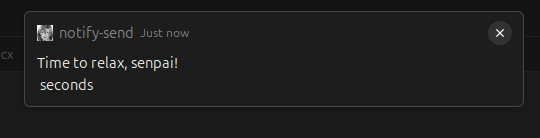
\includegraphics[width=0.95\textwidth]{results/image1.png}
  \caption{Уведомление начала отдыха}
\end{figure}
\begin{figure}[H]
  \centering
  
\includegraphics[width=0.95\textwidth]{results/image3.png}
  \caption{Уведомление окончания отдыха}
\end{figure}
\begin{figure}[H]
  \centering
  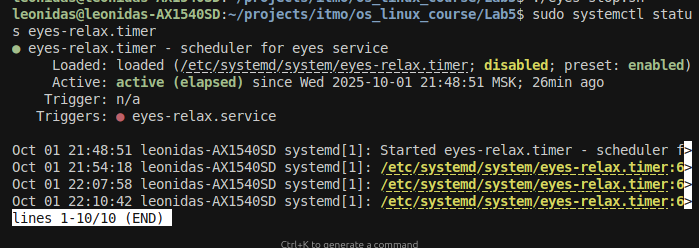
\includegraphics[width=0.95\textwidth]{results/status1.png}
  \caption{Статус юнитов (таймер/сервисы) 1}
\end{figure}
\begin{figure}[H]
  \centering
  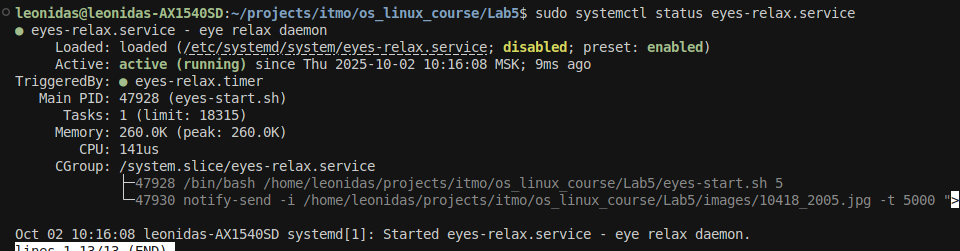
\includegraphics[width=0.95\textwidth]{results/status2.png}
  \caption{Статус юнитов 2}
\end{figure}
\begin{figure}[H]
  \centering
  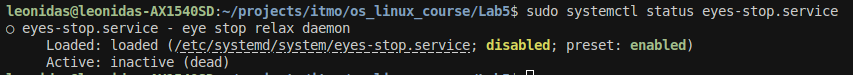
\includegraphics[width=0.95\textwidth]{results/status3.png}
  \caption{Статус юнитов 3}
\end{figure}
                                     % Введение
% \input{3_chap1}                                     % Первая глава
% \input{4_chap2}                                     % Вторая глава
% \input{5_chap3}                                     % Третья глава

\printbibliography[title=Список использованных источников] % Автособираемый список литературы

\end{document}